\documentclass[
  12pt, % Fontsize
  a4paper, % papersize
  %twoside, % For twosided documents
  oneside,
  %openright, % Chapters start always at a odd page
  numbers=noenddot, % No final dots in Sectionnumbers, e.g 1.2 instead of 1.2.
  BCOR=5mm, % Correction length for lost space from binding
  parskip=half*, %No indent but spacing between paragraphs
  thesis
]{bfhbook}

\usepackage{pdfpages}
\usepackage{biblatex}
\bibliography{bib}

% Test Template for bfhbook.cls
\usepackage[T1]{fontenc}
% Coding 
\usepackage[utf8]{inputenc}
% Language setting
\usepackage[english]{babel}

% For more sophisticated blindtext, including lists, math text, etc.
\usepackage{blindtext}

% \usepackage{fonttable}
% Hyperref
\usepackage[                
  % pdftex,                  % for PDF
  colorlinks=true,         % colored links
  linkcolor=black,         % color for links
  citecolor=black,         % color for references
  urlcolor=black,          % color for url 
  bookmarks=true
]{hyperref}              

\usepackage[acronym,toc]{glossaries} % Generate Glossaries
\usepackage{booktabs} % For nicer tables
\usepackage{threeparttable} % Table-Captions having the same width than the table
\usepackage[singlelinecheck=off]{caption}
\usepackage{siunitx} % Scientific Units and number setting
\usepackage{listings} % For Program-Code

%%%%%%%%%%%%%%%%%%%%%%%%%%%%%%%%%%%
% Settings 
%%%%%%%%%%%%%%%%%%%%%%%%%%%%%%%%
% Type?? (Lecture Notes, BSc Thesis, Master Thesis, . . .) 
% Use Variables \BSc, \Master, etc. for language support
\type{Semester project, Game Theory (BTI7501p) '21}
% Author(s)
\author{Alexandre Moeri [moera1@bfh.ch] Kevin Amalthas [kevin.amalathas@students.bfh.ch] Markus Joder [jodem1@bfh.ch]}
% Title
\title{Three men's morris bot}
% Short Title, will be used in the footline
\shorttitle{Three men's morris bot}
% Subtitle
\subtitle{An exploration of search based bots to play the board game "Three men's morris"}
% Titlepicture
\titlepicture{titlepicture.png}
%%

% Topic of Study
\degreeprogramme{Computer Science BSc}
% Supervisor
\thesisadvisor{Prof. Dr. Jürgen Eckerle}
% Version
\version{1.0}
% Date
\date{\today} % Or any other possible date
% Departement
% Use Variable for language support
%\TI

% Semester
% Use Variable for language support
%\semester

% Logo(s)

% Colors
% Secondary Color for Graphics, Tables etc.
% Naming: BFH*Color*light|middle|dark, e.g. BFHGreendark, BFHBluelight, etc.
% Possible Color Values: Green, Blue, Purple, Brown 
\newcommand{\seccolor}{BFHLightBlue} 

\setcounter{secnumdepth}{4}
\setcounter{tocdepth}{4}

\makeindex
\makeglossaries

\begin{document}
\maketitle
%**************************************************************************
\frontmatter % preliminary parts
%**************************************************************************
% Allows breaks in Math Formulars
\allowdisplaybreaks

\tableofcontents
\sloppy
%%%%%%%%%%%%%%%%%%%%%%%%
% Introduction
%**************************************************************************
\mainmatter % The main part
%**************************************************************************
%\part{Part One}
%\chapter*{Management Summary}
%My management summary
\chapter{Introduction}
This report describes our sememster project conducted as part
of the Game Theory lecture (BTI7501p) at BFH.
The goal is to implement a simple game and several
bots using different search based or other approaches.
For our purposes we decided to go with the ancient
strategy board game three men's morris.

\section{Three men's morris}
Three men's morris is an abstract strategy game played on a three by three board
(counting lines) that is similar to tic-tac-toe \cite{wiki}.
The game is also known in the german speaking world as "Römische Mühle" (engl. roman mill)
as it is reported to have been a popular game within the roman army \cite{romanmill}
even though its origins date back to 1400 BCE \cite{threemensmorris}.
It can further be described as a smaller and simplified version of nine men's morris,
also known as "Mühle" in German respectively "Nünistei" in Switzerland,
the still today very popular game - in the Region of Bern especially.

\subsection{Rules}
Each player has three pieces.
The winner is the first player to align their three pieces on a line drawn on the board.
There are 3 horizontal lines, 3 vertical lines and 2 diagonal lines.
The board is empty to begin the game \ref{fig:emptyboard}, and players take turns placing their pieces on empty intersections.

Once all pieces are placed (assuming there is no winner by then), play proceeds with each player moving one of their pieces per turn.
A piece may not move to any vacant point, but only to any adjacent linked empty position, i.e. from a corner to the middle of an adjacent edge, from the middle of an edge to the center or an adjacent corner, or from the center to the middle of an edge \cite{wiki}.

\begin{figure}[hbt!]
  \begin{center}
    \captionsetup{justification=centering}
    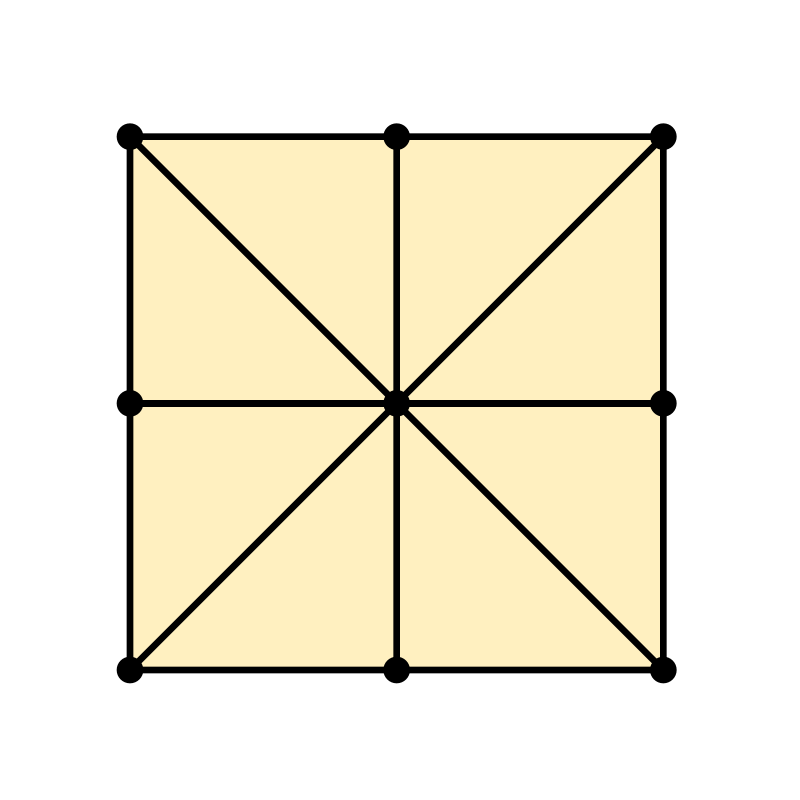
\includegraphics[width=4cm]{emptyboard.png}
    \caption{Empty three men's morris board \cite{wiki-image}}
    \label{fig:emptyboard}
  \end{center}
\end{figure}

\chapter{Method}
\section{Technology}
We took the opportunity to explore some of the newest technologies
and thus the game engine and agents were implemented using an early develepor preview of Python 3.10
\footnote{\url{https://www.python.org/downloads/release/python-3100a7/}}.

\section{Game Engine}

\section{Agents}
\begin{enumerate}
	\item Enum 1
	\item Monte Carlo Tree Search
\end{enumerate}

\textit{Italic text}
\textbf{Bold Text}

\subsection{Monte Carlo Tree Search}
For the Monte Carlo tree search, we followed the fundamental principle in implementing the heuristic search algorithm. Each round of evaluation of the best possible move consists of four steps:
\begin{itemize}
    \item Selection
    \item Expansion
    \item Simulation
    \item Backpropagation
\end{itemize}
In our implementation, we try to follow the steps mentioned above.

The basic functionality of our algorithm is to play a given number of simulations until a winner is determined. During the simulation phase, a score is kept for every simulation, which defines the move's efficiency for the AI to win. Afterwards, the best possible action, based on the highest score, is then chosen and returned.                                     
%\lstset{language=Python}
%\begin{lstlisting}
%from random import stuff
%awesome_python_code()
%\end{lstlisting}
<
\chapter{Results}
\section{Tournaments}
To verify how well each bot performs, we have the different agents compete against each other in a tournament. To get a reference on whether a bot is reasonably configured, we also let a random bot compete in each case, which makes arbitrary moves. It is clear that all bots should clearly win against this agent. To get a meaningful result, we let the bots face each other 1000 times in each encounter.

\subsection{Participating bots}
Monte, Minimax (Reader+Minimax ?), Random

\subsection{Best guess configuration}
In a first pass, we tried to obtain a solid configurations of the bots through empirical observation. For Minimax we found a maximum depth of 7 (d7) and for Monte Carlo a maximum number of simulations of 1'000 (s1000) as a reasonable basic configuration.

We let the bots with these basic configuration compete against each other:

\begin{table}[ht]
  \renewcommand{\arraystretch}{2}
  \arrayrulecolor{white}
  \begin{center}
    \rowcolors{1}{\seccolor!10}{\seccolor!10}
    \begin{threeparttable}
      \begin{tabular}{c|c}
        \rowcolor{\seccolor!50}
        Matchup & Result \\\bfhmidline
        Random vs Minimax (d7) & 0 : 1000 \\\bfhmidline
        Random vs Monte (s1000) & 304 : 696 (7:23) \\\bfhmidline
        Minimax (d7) vs Monte (s1000) & 1000 : 0 \\\bfhmidline
      \end{tabular}
      \caption{Basic configuration}
    \end{threeparttable}
    \label{tab:table1}
  \end{center}
\end{table}

\subsection{Minimax with more depth}
We increase the max depth for the Minimax algorithm to 9 and verify if this improves the performance against the other bots.

\begin{table}[ht]
  \renewcommand{\arraystretch}{2}
  \arrayrulecolor{white}
  \begin{center}
    \rowcolors{1}{\seccolor!10}{\seccolor!10}
    \begin{threeparttable}
      \begin{tabular}{c|c}
        \rowcolor{\seccolor!50}
        Matchup & Result \\\bfhmidline
        Random vs Minimax (d9) & 0 : 0 \\\bfhmidline
        Random vs Monte (s1000) & 0 : 0 \\\bfhmidline
        Minimax (d9) vs Monte (s1000) & 0 : 0 \\\bfhmidline
      \end{tabular}
      \caption{Increased max depth for Minimax}
    \end{threeparttable}
    \label{tab:table1}
  \end{center}
\end{table}

\subsection{More simulations for Monte Carlo}
We increase the max depth for the Minimax algorithm to 9 and verify if this improves the performance against the other bots.

\begin{table}[ht]
  \renewcommand{\arraystretch}{2}
  \arrayrulecolor{white}
  \begin{center}
    \rowcolors{1}{\seccolor!10}{\seccolor!10}
    \begin{threeparttable}
      \begin{tabular}{c|c}
        \rowcolor{\seccolor!50}
        Matchup & Result \\\bfhmidline
        Random vs Minimax (d9) & 0 : 0 \\\bfhmidline
        Random vs Monte (s2000) & 0 : 0 \\\bfhmidline
        Minimax (d9) vs Monte (s2000) & 0 : 0 \\\bfhmidline
      \end{tabular}
      \caption{Increased max simulations for Minimax}
    \end{threeparttable}
    \label{tab:table1}
  \end{center}
\end{table}


\begin{table}[ht]
  \renewcommand{\arraystretch}{2}
  \arrayrulecolor{white}
  \begin{center}
    \rowcolors{1}{\seccolor!10}{\seccolor!10}
    \begin{threeparttable}
      \begin{tabular}{lll}
        \rowcolor{\seccolor!50}
        1 & 2 & 3 \\\bfhmidline
        1 & 2 & 3 \\\bfhmidline
        1 & 2 & 3 \\\bfhmidline
        1 & 2 & 3 \\
      \end{tabular}
      \caption{Table caption}
    \end{threeparttable}
    \label{tab:table1}
  \end{center}
\end{table}

\chapter{Discussion}
\section{Conclusion}
Three men's morris was a simple enough game to implement quickly and get acquainted with the different algorithms that were to be studied in this course.
Due to the nature of the game, especially it's low complexity, the minimax approach has shown to be the most useful, since at relatively low depth winning sequences can be found, and as seen previously even a winning strategy was found for player one.
Minimax is, due to it's simple implementation, relatively slow. It was thus interesting to explore other options and as can be seen in our results the monte carlo approach also renders useful results, at a much faster speed.
Lastly, our current assumption is that, when player 1 does not follow the winning strategy there is always potential for an endless game, that will at some point repeat, when both players refuse to play into a loosing line.

\section{Outlook}
There are several potential optimization that could be made to the project, especially the minimax implementation could be improved on by on one side caching the board state, which would be estimated to already dramatically improve the speed, as well a implement a paralleled version of the algorithm, which would be able to take advantage of multiple core machines and thus also render results faster.
It is thus remains to be seen whether player 2 has winning strategies if player 1 does not start with the center stone.

\section{Sources}

The entire projects source code can be found at \url{https://github.com/amoeri/three-mens-morris}.

\backmatter
% List of Figures
\addcontentsline{toc}{chapter}{Figures}
\listoffigures
% List of Tables
\addcontentsline{toc}{chapter}{Tables}
\listoftables
% Glossary
%\printglossary
% Bibliography
\addcontentsline{toc}{chapter}{Bibliography}
\printbibliography

\end{document}
